\section{Cost Optimization in \sys{}}
\label{sec:optimization}

%\ion{I do not think we need to say "offline" here since we do this optimization per transfer. "Offline" might refer to precomputing a set of possible multicast trees for any possible transfer. The only thing we do not do is recomputing the multicast tree during transfer.}
We design an optimizer to minimize replication cost while meeting a replication time SLO (i.e., a constraint on the maximum replication time to a destination).
Our optimizer has two main contributions.
The first is a Mixed-Integer Linear Program (MILP) formulation of the cost-aware multicast problem, jointly selecting overlay nodes and replication trees. 
% \joey{I rewrote the red sentence below as this sentence:}
% While others~\cite{zhang2018bds} have formulated multicast overlays as MILPs, our approach is fundamentally different both in our objective (cost rather than throughput) and the corresponding framing of the MILP (the space of decision variables).
% sarah: so technically some do model cost
%%% \textcolor{red}{ %\joey{old version}
While others~\cite{zhang2018bds, ganguly2005fast} have used MILP formulations for multicast overlay design, they formulate the optimization problem in terms of \textit{bandwidth}.
Extending these formulations to accommodate per-GB costs would violate linearity as data transfer volume (cost) is proportional to the product of the key decision variables: allocated bandwidth and replication time.
As a consequence, we propose a  new formulation that reframes the optimization in terms of data volume. 
Our new formulation assigns discrete subsets of data (i.e. stripes) to replication paths in the network while ensuring that a complete copy of the data arrives at all destinations.
Unfortunately, solving this MILP formulation can be intractable for larger numbers of destinations.
Our second contribution is an approximation of the MILP formulation that significantly reduces solve time without significantly degrading the solution quality.



\newcommand{\flowmax}[0]{\small{\textsc{bandwidth}}^{path}}
\newcommand{\volume}[0]{\textsc{volume}}
\newcommand{\connectionlimit}[0]{\small{\textsc{Limit}}^{conn}}
\newcommand{\frob}[2]{\langle #1, #2 \rangle}

\newcommand{\dest}[0]{\small{\textsc{dest}}}
\newcommand{\node}[0]{\textit{VM}}
\newcommand{\capacitye}[0]{\small{\textsc{capacity}^\textit{path}}}
\newcommand{\capacityiegress}[0]{\small{\textsc{egress}^\node}}
\newcommand{\capacityiingress}[0]{\small{\textsc{ingress}^\node}}
\newcommand{\capacityvmegress}[0]{\small{\textsc{vmegress}^\node}}
\newcommand{\capacityvmingress}[0]{\small{\textsc{vmingress}^\node}}
\newcommand{\maxinstances}[0]{\textsc{limit}^\node}

% costs 
\newcommand{\coste}[0]{\small{\textsc{cost}}^\textit{path}}
\newcommand{\costi}[0]{\small{\textsc{cost}}^\node}

\newcommand{\runtime}[0]{\small{\textsc{time}}}
\newcommand{\bw}[0]{\small{\textsc{Bandwidth}}^{path}}
\newcommand{\stripes}[0]{\textsc{stripes}}

% variables 
\newcommand{\indicator}[0]{P}
\newcommand{\instances}[0]{N}
\newcommand{\flow}[0]{F}

% constants
\newcommand{\size}[0]{\small{\textsc{transfer-size}}}
\newcommand{\stripesize}[0]{\small{\textsc{size}_\textsc{stripe}}}

% symbol table
\begin{table}[t]
\small
\centering
\resizebox{\linewidth}{!}{
\begin{tabular}{ll}
\toprule
\multicolumn{2}{c}{\textbf{Inputs}} \\

$\size \in \mathbb{R}$ & \textit{Transfer size in GB} \\ 
$\runtime \in \mathbb{R}$ & \textit{Replication time constraint} \\ 
$\stripes \in \mathbb{Z}_+$ & \textit{Number of data stripes} \\ 
\multicolumn{2}{c}{\textbf{Decision Variables}} \\
$\indicator \in \{0, 1\}^{|\stripes| \times |V| \times |V| }$ & \textit{Path indicator variable} \\ 
$\instances \in \mathbb{Z}_+^{|V|}$ & \textit{Number of VMs per region} \\  
$\flow \in \mathbb{R}_+^{|\stripes+1| \times |V| \times |V| }$ & \textit{Flow feasibility variable} \\
\multicolumn{2}{c}{\textbf{Constants: Cross-Region Paths (edges)}} \\ 
$\flowmax \in \mathbb{R}_+^{|V| \times |V|}$ & \textit{Bandwidth profile matrix (Gbps)} \\ $\coste \in \mathbb{R}_+^{|V|}$ & \textit{Network cost (\$/Gbit)} \\ 
\multicolumn{2}{c}{\textbf{Constants: VM Instances (nodes)}} \\ 
% $\capacityiegress \in \mathbb{Z}_+^{|V|}$ & \textit{Per VM egress limit} \\
% $\capacityiingress \in \mathbb{Z}_+^{|V|}$ & \textit{Per VM ingress limit} \\ 
$\capacityiegress\in \mathbb{R}_+^{|V|}$ & \textit{Per region per VM egress limit (Gbps)} \\
$\capacityiingress \in \mathbb{R}_+^{|V|}$ & \textit{Per region per VM ingress limit (Gbps)} \\ 
$\costi \in \mathbb{R}_+^{|V|}$ & \textit{Per region per VM cost (\$/s)} \\ 
$\maxinstances \in \mathbb{Z}_+^{|V|}$ & \textit{Max number of VMs per region} \\ 
\bottomrule
\end{tabular}
}
\caption{Symbol table for \sys{}'s ILP formulation. }
\label{tab:symbols}
\end{table}


\subsection{Egress Cost Minimization Algorithms}
The challenge with our optimization problem stems from having to consider \textit{both} throughput and cost. Without replication time constraints, we observe that the Steiner Tree \cite{hwang1992steiner} minimizes egress cost. 
A Steiner Tree is a set of cost-minimizing edges that form a tree that connects a subset of nodes within a graph. 
If we do not allow the use of waypoint regions, the cost-minimizing tree is a Minimum Spanning Tree (MST).  
 While solving for the MST can be done in linear time, the Steiner Tree problem is NP-hard, though many approximations exist \cite{DBLP:conf/ipco/RehfeldtK21}. 
We cannot use the Steiner Tree to account for replication throughput or instance costs, since it only optimizes total edge cost, but we expect our optimizer's solution to be similar to a Steiner Tree in cases where the replication time constraint is loose. 
%Unfortunately, the classic Minimal Spanning Tree and the Steiner Tree problem formulations only address price. These algorithms are agnostic to available bandwidth per edge, thus can lead to significant slowdowns in data replication. 
%
%In addition, these classic algorithms do not account for resource constraints like per VM ingress and egress limits. They also fail to utilize resource elasticity (i.e., the number of VMs placed in each region) in the cloud to scale the transfer. 

\subsection{Profiling Cross-region Bandwidth}
\label{ss:profiling}
The bandwidth of paths between cloud regions (both intra-cloud and inter-cloud) is determined by the number of VMs in each region, each VM's egress and ingress limits, and the profiled bandwidth. 
As discussed in \cref{ss:bandwidth-variability}, cross-region bandwidth per VM can be estimated by profiling the bandwidth between region pairs using \texttt{iperf3}.
%
Egress and ingress limits vary across cloud providers but are static and can be determined by cloud providers' documentation~\cite{aws_egress_pricing,azure_egress_pricing,gcp_egress_pricing}.
%
%Prior work demonstrates that inter-cloud network bandwidth is stable over 24-hour periods~\cite{jain2022skyplane}, thus 
We utilize these profiles as an estimate of expected network bandwidth for the duration of a transfer. Profiling results are included as part of our open-source repository and shared across all users of \sys{}. 
%\sarah{at some point say: We define the throughput of a distribution tree to be the minimum flow from the source to any destination}

% Cross-region bandwidth can vary dramatically depending on the region pair. We show the distribution of bandwidth (Gbps) groups by each cloud provider pair in \ref{fig:tp_heatmap}. The bandwidth depends on both the VM egress limit and the path bandwidth. For example, AWS caps all cross-region VM egress to 5 Gbps, so outgoing paths from AWS regions are upper-bounded by this limit. Although intra-cloud bandwidth is typically higher than inter-cloud bandwidth, this is not always the case, as there is significant variability in each category. 

%We model the throughput of a data distribution tree given the transfer bandwidth between every region pair and per-VM egress and ingress limits. We profile the transfer bandwidth between all pairs of regions with a single VM as in \cite{jain2022skyplane}. Network egress and ingress limits are determined by the cloud provider. For example, AWS limits cross-region egress of a single VM to 5 Gbps while Azure is unlimited. \shu{reasoning for that} In our setup, we assume that cross-region throughput is a linear function of the number of VMs - i.e. doubling the number of VMs doubles the network egress constraint and cross-region throughput. However, this obviously has a limit because the cloud providers impose extra user-level constraints on the number of VMs that can be created per region. Therefore, we also model throughput in terms of the number of available VMs per region.

%This is particularly problematic in the multicast setting, where source bandwidth is often the constraint.  

%\joey{At this point I don't know anything about egress or ingress limits or inter-region bandwidth flexibility from elasticity.  This needs to be set up more clearly earlier.  This setup could go in 2 or it could go at the beginning of this section as a deeper dive into the problem.}

\subsection{Optimizing Cost with Time Constraints}
\label{sec-optimizer}

\begin{figure}[t]
     \centering
     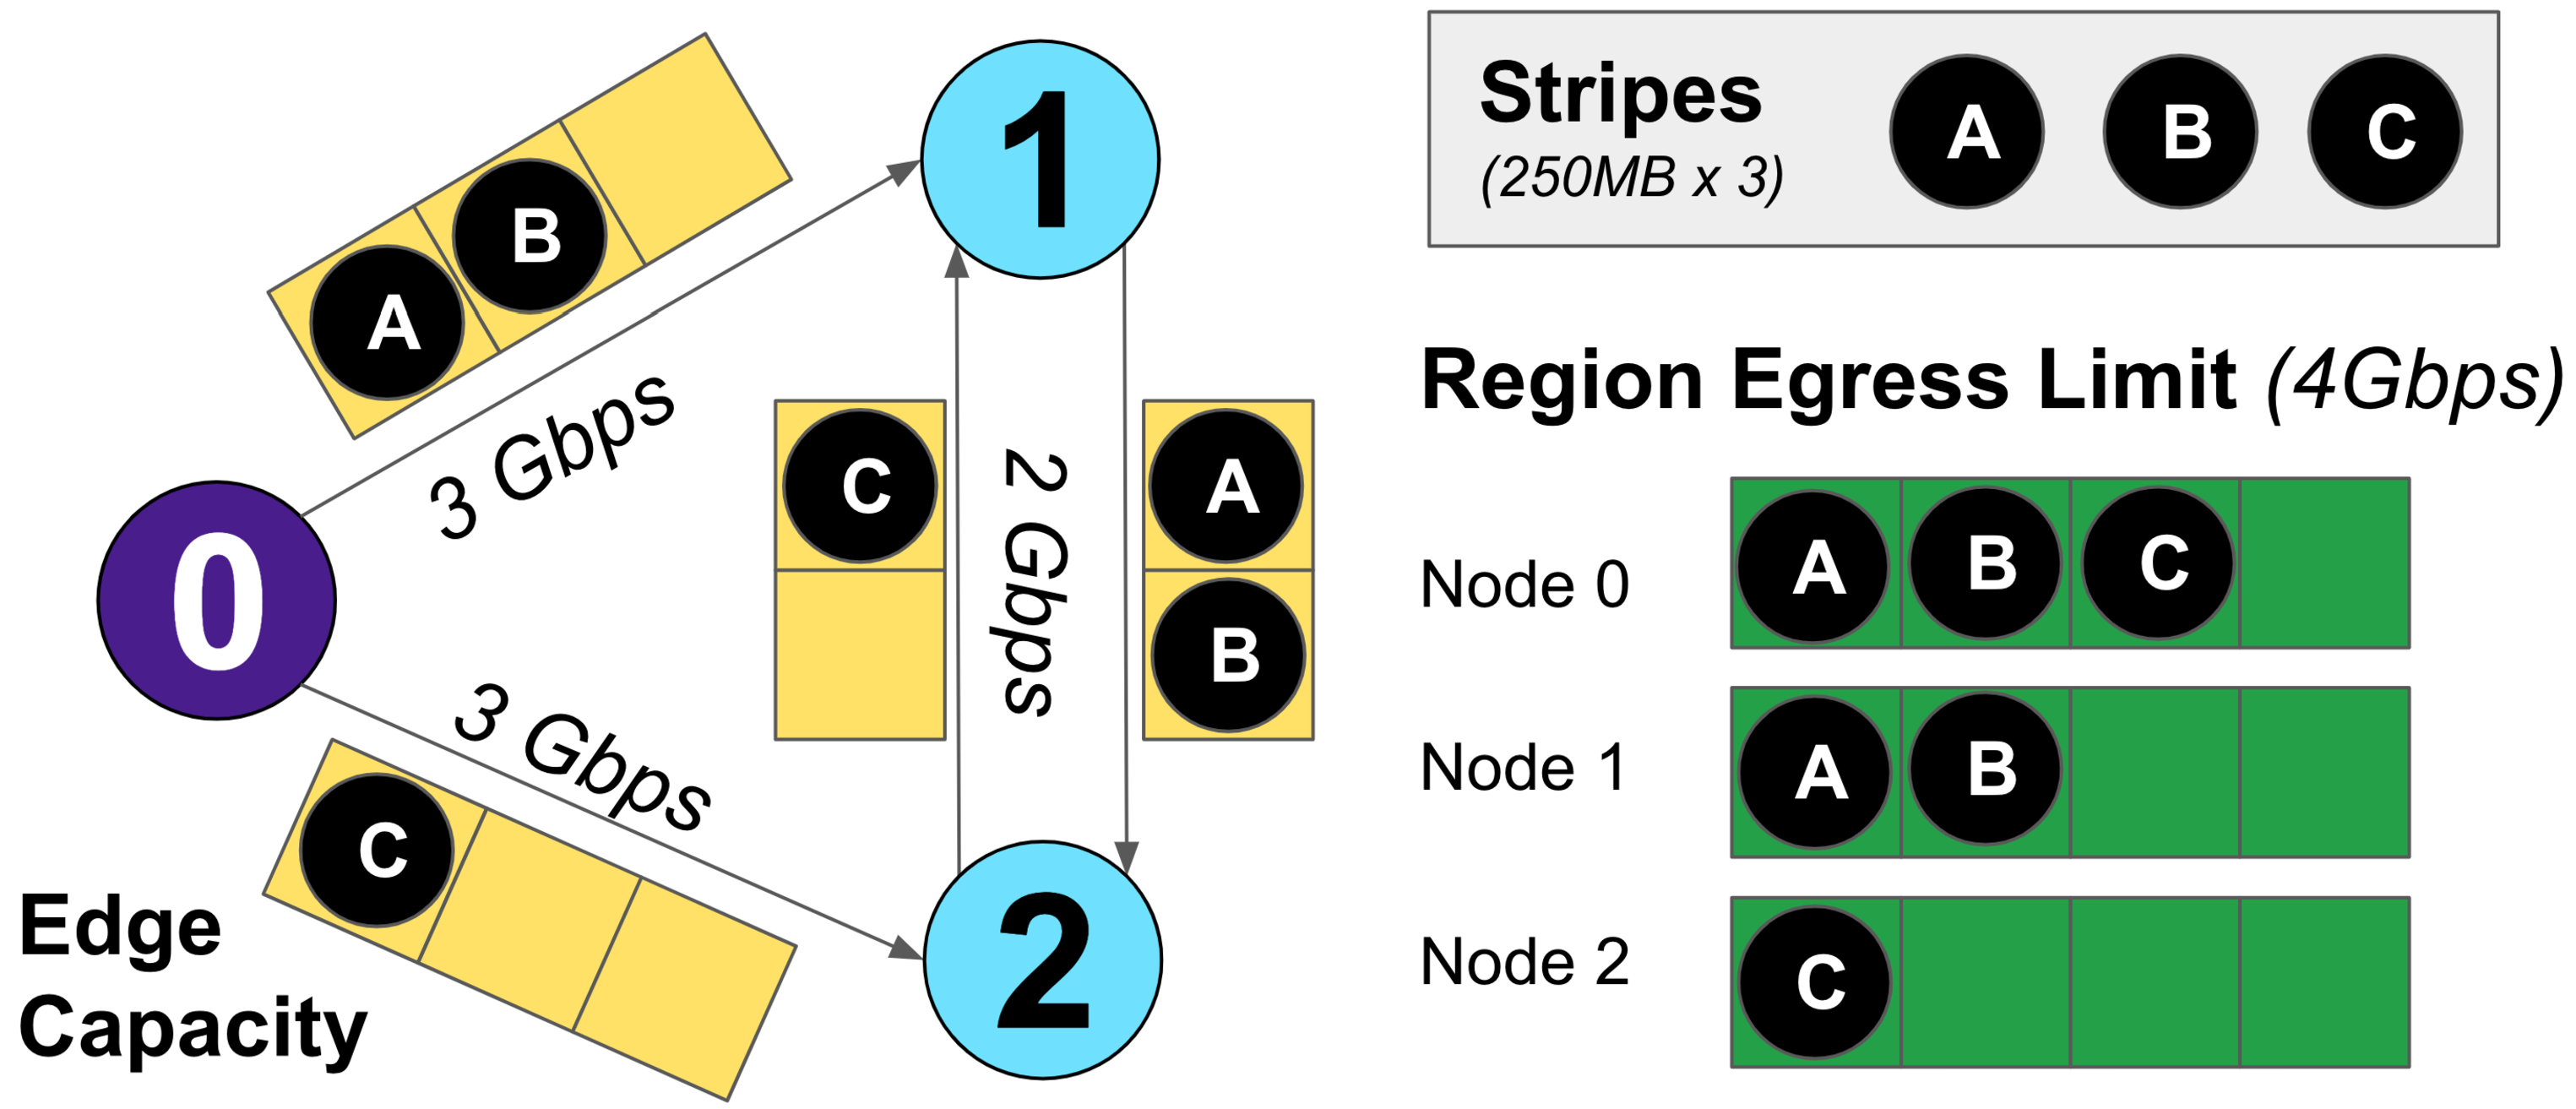
\includegraphics[width=0.8\linewidth]{figures/solver_overview.pdf}
     \caption{Stripes transferred from the source (purple) to destinations (blue) are placed by the solver along edges depending on edge capacity (yellow) and node capacity (green).}
     \label{fig:solver}
\end{figure}

% In order to minimize replication price while still meeting the runtime requirements and cloud resource constraints, we frame a MILP on top of a directed graph that represents the entire cloud topology. The input to the optimizer is the transfer size: $\size$, the runtime budget: $\runtime$, and the number of stripes: $\stripes$, where each stripe is a partition of the data that is routed along the same path. 

% We formulate the MILP in terms of how \textit{stripes} of data are allocated across cross-region paths, rather than throughput. 
% %
% Previous formulations allocate throughput to different edges in the network \cite{castro2003splitstream, zhang2018bds, ganguly2005fast}, which determines the overall throughput and latency of the multicast replication. However, to account for cloud pricing, which is charged per GB, we need to compute the number of bytes transferred along each edge. This introduces a non-linearity in the throughput formulation, as volume of the data transferred is the throughput allocated to the edge multiplied by the replication runtime. 

% In order to formulate the optimization problem as a MILP, we model the optimization problem in terms of allocating \textit{volume} to edges rather than throughput, where the units of allocation are per stripe. We translate cross-region bandwidth and per-region egress/ingress limits into volume capacities,
In order to minimize replication price while meeting runtime requirements and cloud resource constraints, we frame a MILP on a directed graph representing the entire cloud topology. The input to the optimizer is the transfer size: $\size$, the runtime budget: $\runtime$, and the number of stripes: $\stripes$ to divide the data into.

%We formulate the MILP concerning \textit{stripes} of data allocation across cross-region paths, rather than throughput.
%
%Previous formulations allocate throughput to different network edges \cite{castro2003splitstream, zhang2018bds, ganguly2005fast}, determining the overall throughput and latency of multicast replication. However, to account for cloud pricing, charged per GB, we need to compute the number of bytes transferred along each edge. This introduces non-linearity in the throughput formulation, as the data transfer volume is the throughput allocated to the edge multiplied by the replication runtime. 

To formulate the optimization problem as a MILP, formulate the problem in terms of allocating data \textit{volume} to edges rather than bandwidth, with allocation units per stripe. We translate cross-region bandwidth and per-region egress/ingress limits into volume capacities, as shown in \cref{fig:solver}, this determines how many stripes can fit along each edge. This makes the MILP similar to a bin packing problem, where we aim to pack stripes into edges such that all destinations receive all stripes. 
The volume-based representation allows cost to be computed as a function of the number of stripes placed on each edge. 

Next, we formally describe the MILP decision variables, objectives, and constraints. The cloud regions and cross-region paths are represented as $G=(V, E)$, where $V$ denotes the set of cloud regions and $E$ denotes paths between regions. We provide a reference table for the notation in \cref{tab:symbols}.

% as shown in Figure \ref{fig:solver}, which determines how many stripes can fit along each edge. This makes the MILP similar to a bin packing problem, where we want to pack stripes into edges such that all stripes are received by all destinations. 
% Furthermore, computing the cost is simplified by a volume-based representation since we can compute the egress cost from the number of stripes placed on each edge. 

% Next, we formally describe the MILP decision variables, objectives, and constraints. The cloud regions and cross-region paths are represented as $G=(V, E)$, where $V$ denotes the set of cloud regions and $E$ denotes paths between regions. We provide a reference table for the notation in \cref{tab:symbols}.

\subsubsection{Decision variables}

The MILP formulation consists of three decision variables. The path indicator variable $\indicator_{s, (v, u)}$ indicates whether a stripe $s$ is sent between regions $(u, v) \in V$. The paths selected by $\indicator$ make up the multicast replication tree for each stripe. The decision variable $\instances_v$ represents the total number of overlay routers in the region $v$. An additional flow variable $\flow_{s, (u,v)}$ ensures valid paths when constructing the multicast tree. 
It ensures that the paths selected by $\indicator$ do not contain cycles and are connected, by allowing flow to be pushed from the source to all destinations for each stripe (see \cref{constraints}).

\subsubsection{Objective: minimizing price under a deadline} \label{reduce_optimizer_runtime}

To minimize the price of a multicast transfer while meeting replication time constraints, we use a two-part objective function. The first part optimizes the number of virtual machines (VMs) per region, represented by $\instances$, and the second part optimizes the distribution trees per stripe, represented by $\indicator$. The objective is formulated as follows:
%
\begin{eqnarray}
    & \argmin_{\indicator,\instances}&  \underbrace{\runtime \times \frob{\costi} \instances}_\text{Instance Cost}  \\ 
    &+& \underbrace{\frac{\size}{\stripes} \times \sum_{s\in{\stripes}}  \frob{\coste} {\indicator_s}}_\text{Egress Cost}
\end{eqnarray}
%
The price of a data transfer is the sum of the instance fee and the egress fee. The instance fee depends on the number of VMs running per region, the job completion time, and the per-region VM fee. The egress fees are determined by the data distribution path and the amount of data traversed through the path, as defined by $\indicator$. We note that the instance cost is also an upper bound as it can be potentially overestimated if the data transfer is completed in less than the user-defined time budget. However, this is necessary to ensure linearity.

\subsubsection{Constraints}
\label{constraints}
We represent cross-region bandwidth, node egress/ingress bandwidth, per-region VM limits, and replication tree structure requirements as constraints within the MILP.

\heading{Representing Inter-Region \& Inter-Cloud Bandwidth} 
Cross-region bandwidth is represented as the \textit{per-GB capacity} given the run-time budget, i.e., how many stripes can fit along an edge. Increasing the number of VMs in the source regions linearly increases the rate at which we can send data. We thus model the bandwidth between two regions as the per-VM bandwidth profiled between those two regions multiplied by the number of VMs in the source region:
% As such, the volume capacity between the two regions is:
% \vspace{-0.1em}
\begin{equation}
    \capacitye = \frob{\instances} \bw * \runtime, 
\end{equation}
% \vspace{-0.1em}
and constrain $\indicator$ in terms of the path capacity: 
% \vspace{-0.1em}
\begin{flalign}
\forall (u, v)\in E 
    && \stripesize * \sum_{s} P_{s,(u,v)} \le \capacitye_{(u, v)}.
\end{flalign}
to ensure allocated stripes fit within the capacity. 

\heading{Representing VM Bandwidth Constraints}
Cloud providers impose per-VM bandwidth constraints on network egress, as described in \cref{ss:bandwidth-variability}. As such, a major bottleneck of multicast transfer is the source region's limited egress bandwidth. 
% 
We constrain $\indicator$ in terms of the ingress and egress limits: 
\begin{flalign} 
 \forall v \in V   &~~ \stripesize * \sum_{s}\sum_{u\in V} P_{s, (v, u)} \\ & ~~~~\le \capacityiegress_v * \instances_v * \runtime \\ 
\forall u \in V &~~ \stripesize * \sum_{s}\sum_{v\in V} P_{s, (v, u)} 
\\ & ~~~~\le \capacityiingress_u * \instances_u * \runtime 
\end{flalign}

\topheading{Representing VM Capacity Constraints}
We account for per region VM limits by adding the constraint $\instances \le \maxinstances$.

% Cloud providers limit the number of VMs that can be created per region, which we account for by adding a constraint $\instances \le \maxinstances$.\

\heading{Ensuring Valid Multicast Trees}
We use an additional variable $\flow$ to ensure that the paths selected by $\indicator$ are valid distribution trees, i.e., they are connected and acyclic, and they deliver all data to each destination. At a high level, we ensure that $\flow_{s, (u, v)}  \ge 1, \text{ if } \indicator_{s,(u,v)} = 1$, and impose conservation of flow constraints on $\flow$ but not $\indicator$, since $\indicator$ is an indicator variable not a flow variable. We then ensure that flow can be pushed from the source node to destination nodes on $\flow$ for each stripe, which also ensures that flow can be pushed from the source to destination for the paths selected by $\indicator$ (without having to impose flow conservation on $\indicator$). We leave details on this part of the formulation for \cref{s:formulation-details} due to space. 

\subsubsection{Solver feasibility}
Our formulation so far has a search space of size $O(2^{|V|^2\times|\stripes|})$. With 71 possible regions across GCP, AWS, and Azure and 10 stripes, the search space is, therefore, $O(2^{50410})$, which is infeasible even for advanced solvers to solve within a few minutes, necessitating approximations. 


% \subsection{ILP Formulation}


% We define a  problem for a set of equally sized partitions over a graph with known throughput and cost parameters over edges: 
% \begin{itemize}
%     \item $C$ = set of partitions (each of equal size $PARTITION\_SIZE$)
%     \item $V$ = vertices in the graph (i.e. regions). 
%     \item $COST_{edge}$ = $|V|\times|V|$, cost per GB of each edge
%     \item $TP_{edge}$ = $|V|\times|V|$, throughput of each edge
%     \item $COST_{instance}$ = $|V|$, cost per second running a VM in a region
% \end{itemize}
% There are three decision variables for the ILP: 
% \begin{itemize}
%     \item $P \in \mathbb{B}^{|C|\times|V|\times|V| }$: A boolean array indicating whether an edge is used to transfer a partition
%     \item $N \in \mathbb{N}^{|V|}$: An integer array indicating the number of VMs per region
%     \item $F \in \mathbb{Z}^{|C|\times|V|\times(|V|+1) }$: An integer array to ensure that for each partition, flow can be pushed along the partition's from the source vertex to all destination vertices. 
% \end{itemize}

% \subsection{Cost minimization}
% We define the objective as cost minimization as shown below: 
% \begin{equation}
%     \min \sum_{c \in C} P_c \times COST_{edge} \cdot PARTITION\_SIZE + N \times COST_{instance} \times s
% \end{equation}
% Given a deadline $s$, our optimization problem can be formulated as follows 
% \begin{gather}
% 	\underset{path, INST}{\text{arg min}}  \sum_{(u,v) \in E} \sum_{k=1}^{n} path_{(u,v),k} * \frac{VOLUME}{n} * COST_{(u,v)} + \sum_{i \in V} INST_i * \text{COST\_INS}_i * s \\
% 	\text {Subject to } \forall t \in D \text{, } \forall k \in \{1,...,n\} \sum_{(u,t) \in E}  path_{(u,v),k} \geq 1 \\
% 	\forall k \in \{1,...,n\} \sum_{(s,v) \in E}  path_{(s,v),k} \geq 1 \\ 
% 	\forall v \in V - \{s\} \text{ ,  }\forall k \in \{1,...,n\} \sum_{(v, w) \in E} path_{(v,w),k} \sum_{(u,v) \in E} path_{(u,v),k}  \geq \sum_{(v, w) \in E} path_{(v,w),k} \\ 
% 	\forall (u,v) \in E \sum_{k=1}^{n} path_{(u,v),k} * \frac{VOLUME}{n} \leq BW_{(u,v)} * s\\ 
%     \forall v \in V \sum_{(u,v) \in E} \sum_{k=1}^{n} path_{(u,v),k} * \frac{VOLUME}{n} \leq \text{vm\_ingress\_lim} * INST_v * s\\ 
%     \forall u \in V \sum_{(u,v) \in E} \sum_{k=1}^{n} path_{(u,v),k} * \frac{VOLUME}{n} \leq \text{vm\_egress\_lim} * INST_u * s
% \end{gather}

\subsection{Reducing Optimizer Runtime}
\label{ss:approximations}

In this section, we describe several mechanisms that we combine to reduce the optimization runtime or an order of seconds, while still maintaining solution quality. 

% \subsubsection{Stripe-Iterative Approximation}
% \vincent{a section with only 1 subsubsection is weird.  Just make everything a paragraph heading?} \shu{add}

\begin{figure}[tbp]
     \centering
     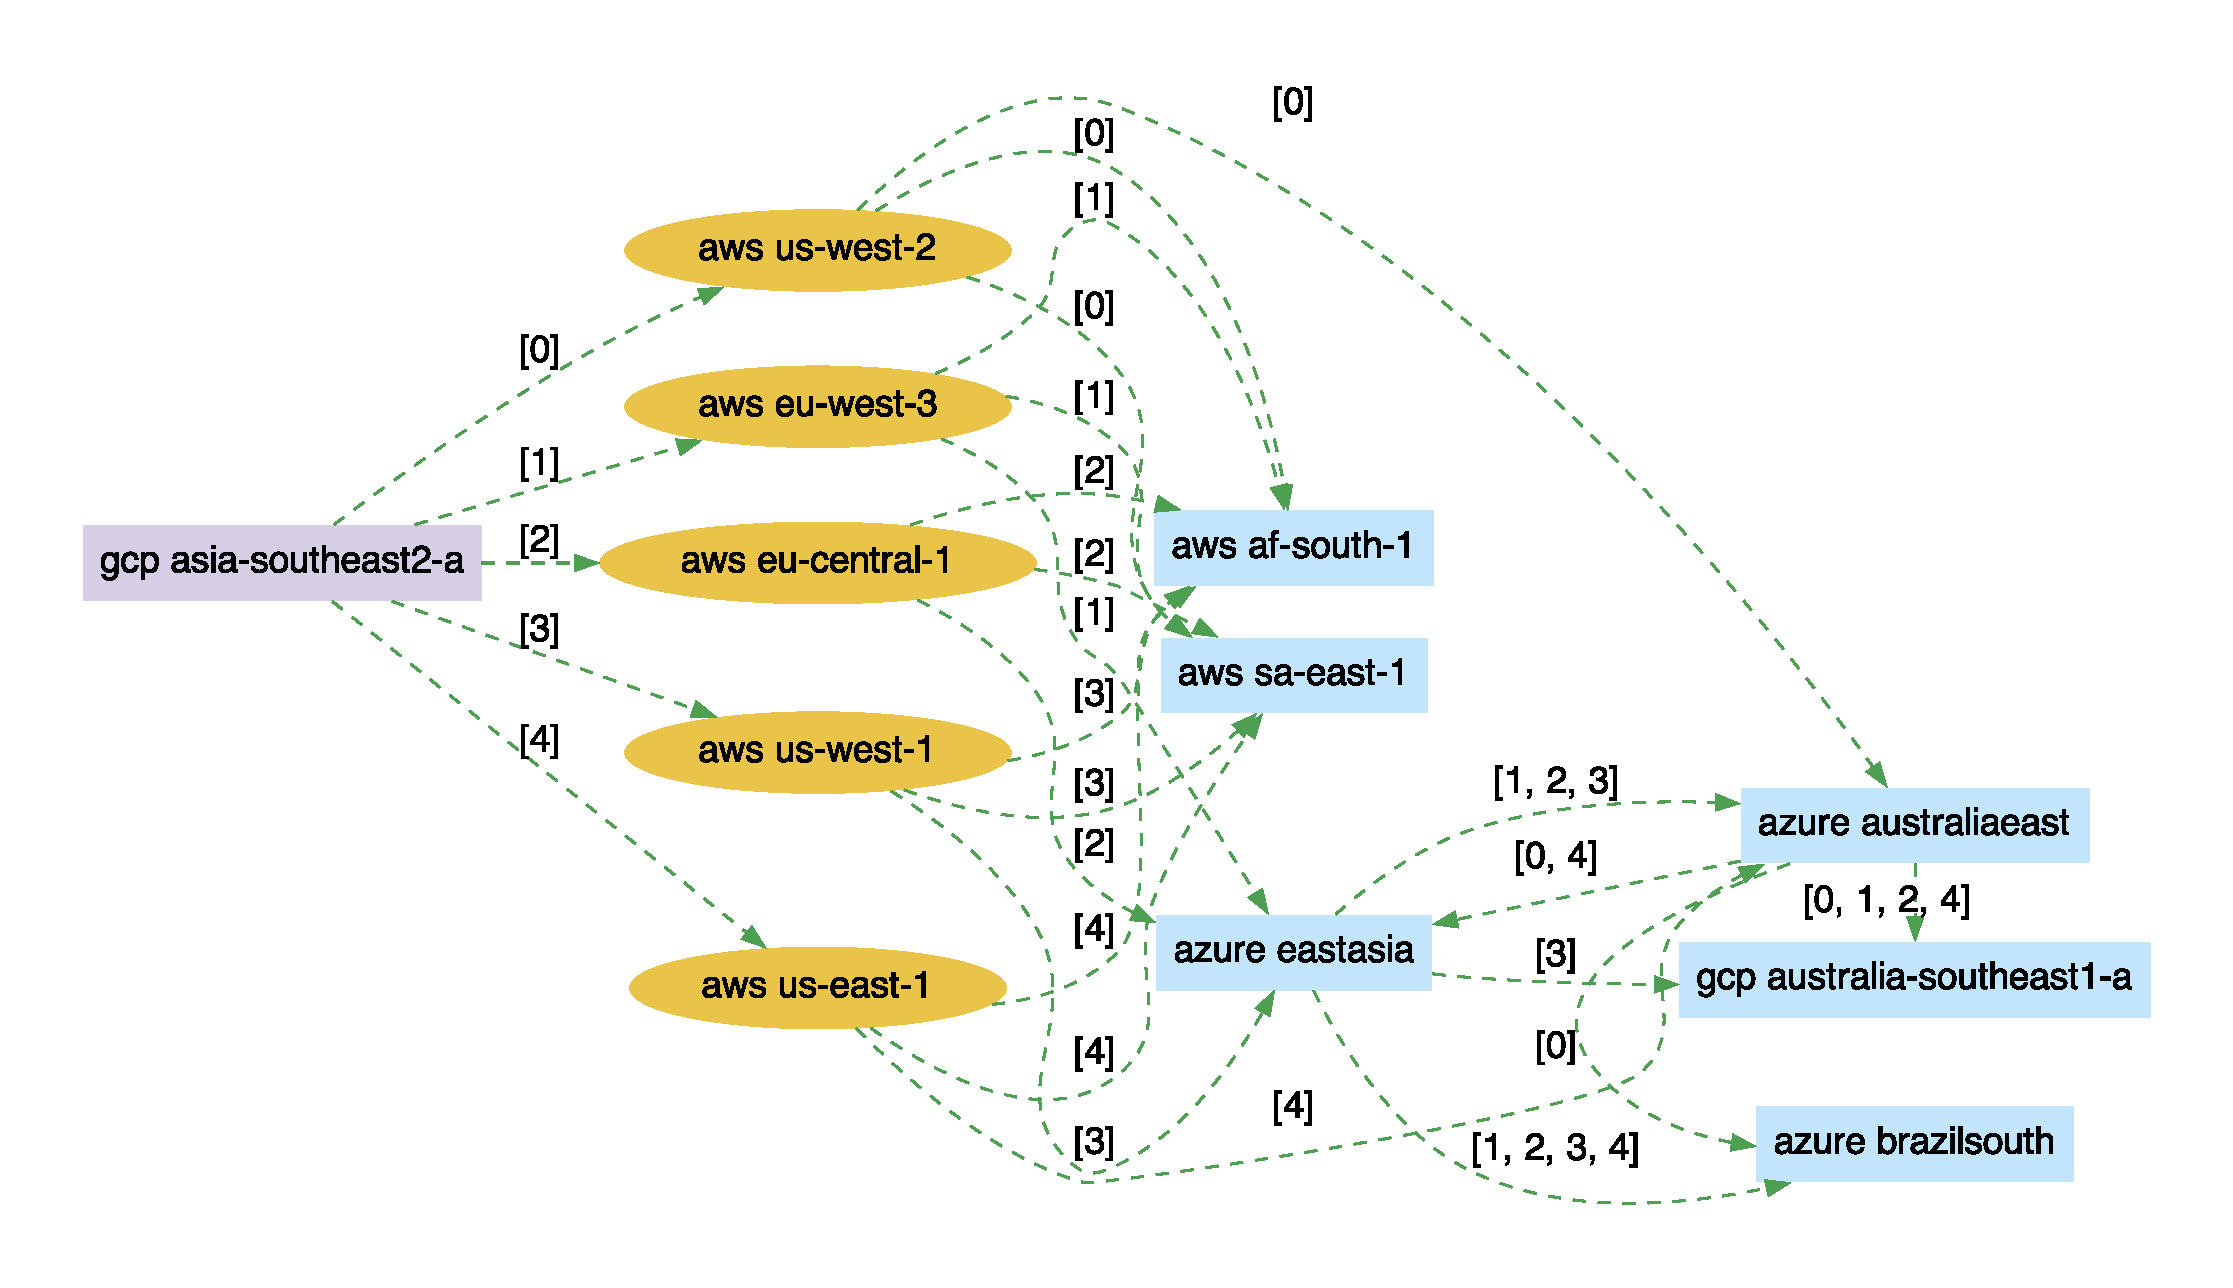
\includegraphics[width=\linewidth]{figures/partitions.pdf}
     \caption{Visualized solver output for inter-cloud replication described in \cref{sec:algorithm_eval}, consisting of source (purple), waypoint (yellow), and destination (blue) regions. The data is divided into 5 stripes (marked on edges). }
     \label{fig:example-topo}
\end{figure}

\heading{Node Clustering}
\label{node-filtering}
We observe that many regions across cloud providers share similar characteristics in terms of bandwidth and the costs of their outgoing and incoming paths. A motivating observation was that sub-sampling regions randomly could produce similar solutions with much lower solve time, as shown in Figure \ref{fig:node_selection}. At a high level, AWS regions in Europe regions all have similar egress/ingress costs and bandwidth, so only one of those regions needs to be considered as a potential waypoint. Therefore, to reduce the optimizer search space, we cluster regions using their incoming and outgoing path costs and bandwidth as features and select a representative node from each cluster. We empirically find that, with about 20 clusters (i.e. 20 subsampled regions), the optimizer can generate solutions that are reliably similar to the original MILP without approximation (more discussion in \cref{sss:solution_qual_eval}). 

%We aim to reduce the problem size and solve time by filtering out regions that may not be helpful in improving the solution quality. Our evaluation in \cref{fig:node_selection} shows that there is a diminishing return of solver solution quality with an increasing number of considered regions. Therefore, we implement node filtering by forming clusters of regions based on their profiled characteristics (e.g., cost, bandwidth) to all other available regions.

%By forming 20 clusters on 71 regions, we can speed up the solving time by a significant margin while maintaining solution quality within a reasonable range from the optimal solution. We select our set of considered regions by sub-sampling a single region from each cluster. Although node filtering carries the risk of reducing optimizer quality by leaving out potentially useful waypoint regions, we observe that there are sets of regions that contribute similarly to solving the multicast data replication tree. For instance, regions in similar geographic locations (e.g., Asia, or North America) might share similar characteristics, and only a small subset of them will be used by the MILP.
% We find out that in practice, forming 20 clusters on 71 regions speed up the solving time by \todo{xx} while still maintaining solution quality within xx\% from the optimal.

\heading{Hop Constraining}
\label{edge-filtering}
To further reduce the optimization space, we only consider a maximum of 2-hop overlay waypoints. Previous research has shown that limited numbers of overlay hops are often sufficient \cite{andersen2001resilient, peter2014one, stoica2002internet}. Our analysis also found solutions using multiple overlay hops to be rare, suggesting that they need not be considered. We implement the hop constraints as an additional constraint on the MILP. 

\heading{Stripe-iterative Approximation} To make the optimizer runtime linear with respect to the number of stripes (rather than exponential), we design a greedy, stripe-iterative approximation algorithm that solves for one stripe per iteration. We solve for each stripe independently, then update the input graph for the next stripe by reducing the path capacity ($\capacitye$), instance limits, and egress/ingress limits per region ($\maxinstances$, $\capacityiegress$, and $\capacityiingress$).

\subsection{Example Topology}
We show an example of the optimizer's output replication tree topology visualized in Figure \ref{fig:example-topo}. Due to variability in cloud provider egress pricing and cross-region throughput, our optimizer often finds unexpected solutions, such as routing one stripe (marked \texttt{[3]}) from GCP to AWS, AWS to Azure, then back to GCP. Although questionable at first glance, we evaluate this same replication in Figure \ref{fig:inter-cloud-1} and demonstrate both cost and replication time improvements over baselines. 
